\section{Introduction}

%% 
%% Leave first page empty
\thispagestyle{empty}

The need of a new way to communicate between two points of the planet has been arising as a problem to be solved by our new media distributors. Traditional systems such Skype or video calls are not able to cope the needs of the new generations of developers and users that everyday require a more integrated way of communication with the World Wide Web (WWW). 

Besides this, the amount of data being transferred during the last years and the prevision for the future allocates a new scenario where non-centralized systems such as P2P are required as data bandwidth grows and systems need to become more scalable. Nowadays, networks are still manly content-centric, meaning that data is provided from a source to a client in a triangle scheme, clients upload data to central servers and this data is transferred to the endpoint. This architecture has been provided since long time as reliable and scalable, but with the appearance of powerful applications and Video On Demand (VOD) it has been proven to become a real problem.

Those circumstances lead to a whole new world of real-time browser based applications which require also a totally new framework to be developed into. Starting from the online videoconferencing to real-time data applications, for this purpose few attempts where made in the past being highly reliable on specific hardware and custom-built no-compatible system. Taking these decisions made those proposals not be accessible by the massive amount of normal users that could not afford to adapt the requirements. 

All the previous concepts are now possible thanks to the increase of performance related to the hardware components available in every average computer nowadays, this increase has helped to build more complex browsers that are able to perform many tasks not just related to web browsing. Having a browser handling OpenGL style of applications is now possible thank to the new HTML5 standard. Multimedia abilities have also been able to be reproduced on those browsers and handling webcam media as HTML is now a reality. Even dough there are still some issues to be considered before being able to freely communicate between two browsers: there is no common standardized protocol that allows developers to do this. WebRTC goal to approach this problem is to build a simple and standard solution for peer-to-peer browser communication \cite{alvestrandOverview2012} in the HTML5 environment.

Internet bandwidth has helped to take the decision to start integrating peer-to-peer solutions in browsed based applications, this is due the year-by-year increase of user bandwidth connectivity during the last 10 years. As before the latency was too high being unable to maintain real-time applications working resiliently. But recently the amount of users being able to transfer at high speed has been rapidly increasing as you can see in Figure ~\ref{fig:bwWorldAvg}, about 39\% of users are now able to download at speeds greater than 4Mbps being this a very good average speed for media content \cite{akamaiq2}.

\begin{figure}[h]
  \centering
    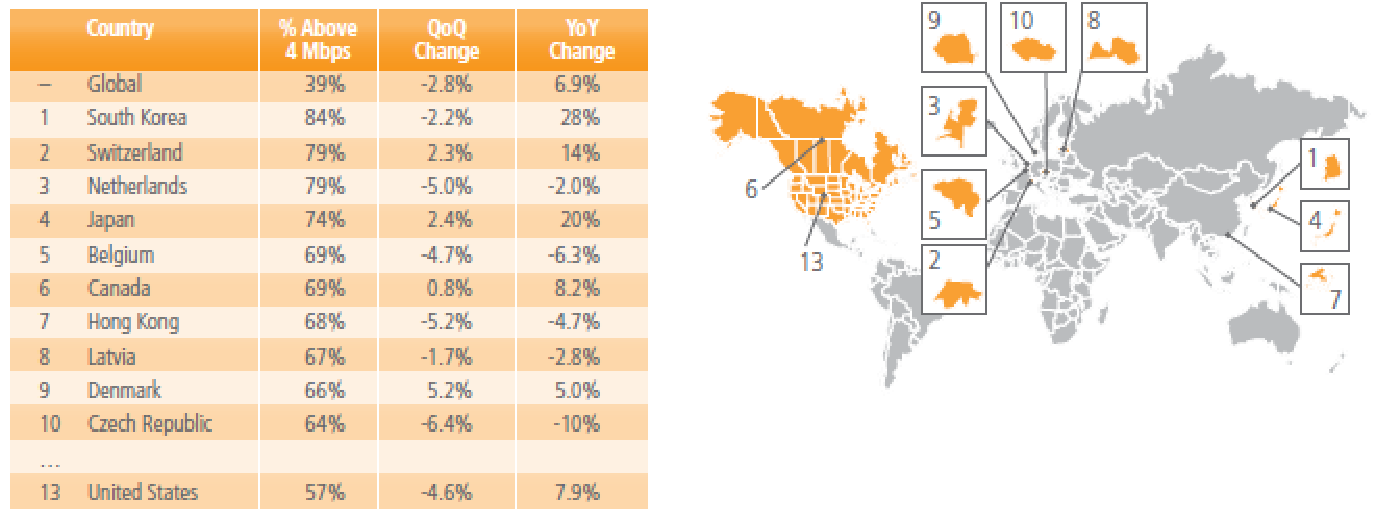
\includegraphics[width=1\textwidth]{./figures/internetstats.pdf}
      \caption[Broadband over 4Mbps connectivity statistics]{Broadband connectivity statistics about the speeds over 4Mbps around the globe.}
	\label{fig:bwWorldAvg}
\end{figure}

Regarding the specs on the client side, recent surveys and statistics taken by the game manufacturer Steam  \cite{steamStats} has proven that nowadays more than  61\% of machines are carrying 1 to 4 gigabytes of RAM and nearly 90\% of computers are handling 2 to 4 core CPU with a 64 bit OS, being this environment optimistic for media enhanced applications which require high performance for video encoding and similar. Due to the layering needed to standardize a system like WebRTC running in top of an underlying application such as the browser that handles many processes is very important to rely on a powerful machine. Usually this was not able to be done in the past and one of the challenges has always been performance. They key to success is always to optimize the performance of a process so it does not affect the user experience, one of the challenges of WebRTC.

Traditionally, this concept of performance was approached by the usage of plug-ins or other separate software components which made the system run smoother by avoiding one layer of processing (browser) but being non-standard and not cross-compatible, one of the most import ant concepts when designing applications nowadays. Now the traditional approach has become outdated with the arrival of the new HTML5 where WebRTC is integrated as one of the new Application Programming Interfaces (API) available alongside other many different interesting capabilities.

%\subsection{History}
%
%Web Real-Time Communication is an API definition with the aim to start an interoperability standard that will help to build P2P applications in the developer layer. The first announcement concept went public in a working group of the World Wide Web Consortium (W3C) in May 2011 \cite{webrtcW3cgroup} and starting the mailing list in April 2011 \cite{welcomeW3C}. During the first stage of the working group the main goal was to define a public draft for the API implementation and a route timeline with the goal to standardize the protocol by ends of 2012. The first public draft of the W3C came public the 27th of October 2011 written by Adam Bergkvist (Ericsson), Daniel C. Burnett (Voxeo), Cullen Jennings (Cisco) and Anant Narayanan (Mozilla) \cite{originalW3Cdraft}. During this first W3C draft only media (audio and video) where considered as candidates to be sent over the network to other peers, manly focusing in the way browsers will be able to access the media devices without using any plugin or external software.
%
%Alongside to the W3C working group the WebRTC concept also joined the IETF with a working group in May 2011 \cite{webrtcIETFgroup} with the first public announcement charter done the 3th of May 2011 by Magnus Westerlund (Ericsson), Cullen Jennings (Cisco) and Ted Hardie (Ericsson). The milestones of the working group charter initially marked December of 2011 to provide the information and elements required to the W3C for the API design input. On the other side, the main goals of the working group covered the definition of the communication model, session management, security, NAT traversal solution, media formats, codec agreement and transport of the data \cite{webrtcIETFcharter}. Those goals have been evolving during the standardization process and the work done along with the W3C working group.
%
%An important point during the process of standardization came the 1st of June 2011 when Google publicly released the source code of their API implementation \cite{haraldpublicWebRTC}. 
%
%During all this period both working groups have been working alongside to provide a reliable solution to enable applications to perform media and data transfer in a plugin-free environment.
%
%\subsection{Support}
%
%The following companies have publicly supported and are actively working in the development of WebRTC standards in the W3C: Google, Mozilla and Opera \cite{googleAnnouncement}. Other companies such as Microsoft have been publicly supporting a browser-to-browser solution but have provided their own proposal which differs with the one published in the WebRTC group called CU-RTC-Web \cite{curtcweb}, this proposal did not get much traction by the workgroup being declined to unify with the current specs, during an W3C workgroup poll in September 2012 the chairs of the group decided to attach the development to the already existing WebRTC API instead of moving it to the CU-RTC-Web \cite{curtcpoll}.
%
%During the firsts attempts to build a reliable solution for WebRTC Ericsson Labs publicly presented an initial API based on the preliminary work done in the Web Hypertext Application Technology Working Group (WHATWG), this API was called ConnectionPeer API and required an special module to be installed in your browser \cite{ericssonwebrtc}. Ericsson lately dropped from the production of it's own browser to focus in the standardization effort and codec discussion leaving the API implementation to the Mozilla and Chrome teams. The original API evolved rapidly during the next months thanks to the workgroup and the developer community feedback thanks to the encourage of the Chrome team to experiment with the unstable API.
%
%
%\subsection{Milestones}
%
%During the process of standardization in WebRTC some important moments should be remarked. In January 2012 Opera implemented the first version of WebRTC getUserMedia for accessing the camera and audio \cite{operaannouncement}, during this year getUserMedia is available in the stable version. 
%
%Google Chrome integrated the first version of WebRTC in its dev and canary channels of the browser during January 2012 \cite{chromeannouncement}, in June 2012 it started moving its API to the stable channel hidden behind a flag, in November 2012 WebRTC becomes fully available in Google Chrome stable channel and is open for user usage \cite{chromestable}. 
%
%Mozilla Firefox started working on the getUserMedia implementation early 2012 delivering the first version of media access trough API at the beginning of 2012 in the alpha version \cite{mozillablog}, in April 2012 Mozilla published a WebRTC video demo running on Firefox in the "adler" channel \cite{mozillawebrtc}, also supporting some primitive DataChannel API. Later in October Firefox Nightly was carrying the first unstable version of the WebRTC API including DataChannel \cite{mozillafinal}, Mozilla announced in September 2012 that the stable version of WebRTC will be shipped along with Firefox 18 in January 2013 \cite{mozillacomming}. 
%
%Some announcements have been done from Microsoft as they are also still working in some implementation into Internet Explorer by using CU-RTC-Web as the default standard, at the moment only the Media API information has been published \cite{microsoftcapture}.
%
%In the mobile environment there has been less efforts than in the desktop browsers. In October 2012 Ericsson announced the world's first WebRTC-enabled browser for mobile devices called "Bowser" with support for iOS and Android, this browser is able to handle WebRTC calls using RTCWeb Offer/Answer Protocol (ROAP) which is an old discontinued version of the WebRTC API that has moved to Javascript Session Establishment Protocol (JSEP). This browser also differs from the previous desktop alternatives on the codec side, it is carrying H.264 for video and G.711 for audio \cite{ericssonbowser}. The provided API for Bowser is not fully W3C compliant yet.
%
%\subsection{Issues in WebRTC}
%
%WebRTC uses a mixture of different technologies to perform peer-to-peer communication between clients, those technologies range from SRTP, RTP, RTCP (in the future) and multiple codecs that are being discussed. This scenario makes performance the key point for success in developing stable WebRTC applications in the near future. 
%
%Performance is manly related to computer capabilities and the ability to encode/decode at the same time as transferring and monitoring multiple peer connections. All those tasks are now run over the browser not directly on the OS, this is good for interoperability between platforms but bad in the performance aspect. 
%
%Media applications are delay sensitive and require a low packet loss for its proper function, WebRTC is working on this trying to implement congestion control over the connection stablished between peers, this work has not been completed yet and will arise as a problem in the near future. Packet loss due to system capacity and bandwidth should be measurable and adaptive in an infrastructure such as WebRTC.
%
%Constraints and bandwidth statistics will make a big difference in how media is performed in WebRTC. Browsers and web applications have been always able to tolerate some amount of delay and packet losses but this is not possible in media infrastructures for real time conversations, a change of scope is needed to be able to handle Quality of Service (QoS) in WebRTC.
\subsection{Background}

WebRTC API is included into the HyperText Markup Language version 5 (HTML5), this is the fifth version of the WWW language. This version includes different API's and JavaScript codes that help the developer to easily introduce new features into their already existing WWW applications. The initial HTML version (2.0) was published in November 1995 \cite{html2IETF} with the only goal of delivering static content from the server to client browser. This language was used since 1990 even the standardization process ended in 1995, with the initial goal of serving data format that is portable to multiple platforms HTML became de de facto format for serving web information. 

HTML is written in form of angle brackets (< >) named tags that contain different elements. Those tags are then interpreted by the browser to show the different data content served by the server. During the evolution of the WWW different new concepts where added to the HTML standard and new versions where published, things like JavaScript and Style Sheets made increased the flexibility and features of the WWW content enhancing the final user experience.

Due to the need of extending the features of the already existing HTML4 standard a new version was proposed in 2004 by the Mozilla Foundation and Opera Software \cite{initialHTML5proposition}. This new proposition was focused in new developing technologies that could be backwards compatible with the already existing browsers, the idea didn't make a success and was tier apart until January 2008 when the first Public Working Draft was published by the Web HyperText Application Technology Working Group (WHATWG) in the W3C \cite{firstHTML5draft}.

This proposal had a greater reliance in modularity in order to move forward faster, this meant that some specs that were included in the initial draft moved to different working groups in the W3C. Those technologies defined in HTML5 are now in separate specifications, one of them being WebRTC. WebRTC works as an integrated API within the browser that is accessible by using JavaScript and is used in conjunction with the Document Object Model (DOM) interfaces. Some of the APIs that have been developed are not part of the HTML5 W3C specification but are included into the WHATWG HTML specification.

\subsection{Contribution}

Investigate how WebRTC performs in a real environment trying to evaluate the best way to set multiple peer connections that are able to transfer media and data in different network topologies. Measure the performance of WebRTC in a real environment trying to identify bottlenecks related to encoding/decoding, media establishment or connection maintenance. All this should be able to be performed in real-time over a browser by using the already existing WebRTC API.

Using metrics related to RTT, latency, packet loss and bandwidth usage we expect to understand the way WebRTC performs when handling multiple connections.

\subsection{Goals}

WebRTC uses and adapts some existing technologies for real-time communication. This thesis will focus in studying how:

\begin{itemize}
	\item WebRTC performs considering different topologies using video acquired by the API itself form the Webcam and encoded using different codec types provided by the standard.

	\item Usage of WebRTC to build a real application that can be used by final users proving that the API is ready to be deployed and is a good approach to the developer needs when building real-time applications over the web. This will be done in conjunction with other new APIs and technologies introduced with HTML5.
\end{itemize}

The final conclusion will cover an overall opinion and usage experience of WebRTC providing some valuable feedback for the needs and requirements for further modifications of the API.

\subsection{Structure}

Not sure about here